\documentclass[12 pt]{exam}
\usepackage{graphicx, enumitem, amsmath, amssymb}
\graphicspath{ {./images/} }
\usepackage{tikz, pgfplots}
\usetikzlibrary{shapes,arrows}
%\usepackage{Minion Pro}
\printanswers

\title{1.5 Preferences II: MRS and Utility Functions - Practice Problems (Answers)}
\author{Ryan Safner}
\date{ECON 306 - Fall 2019}

\begin{document}

\maketitle
 
\begin{questions}

\question For each question, draw an indifference curve relating the two objects (label it $I_1$). Draw and label a *second* curve that gives *higher* utility (label it $I_2$), and a *third* curve that gives *lower* utility (label it $I_0$).

\begin{parts}

		\part 	Oranges (a good) on the horizontal axis and Pollution (a bad) on the vertical axis. 
			\begin{solution}
				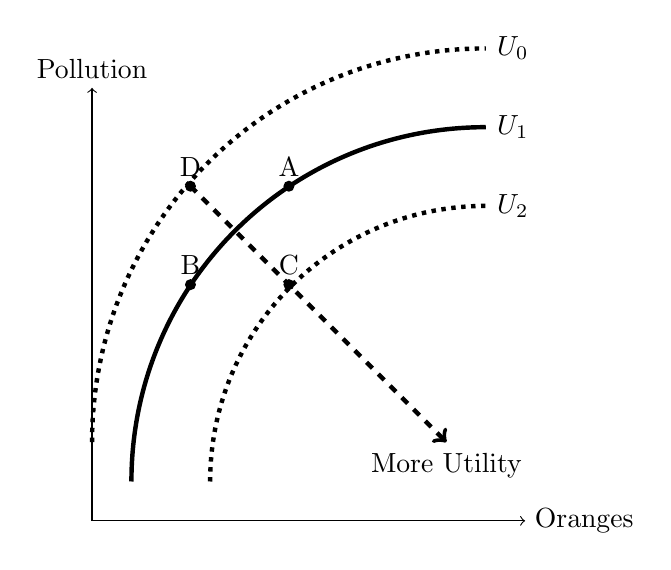
\begin{tikzpicture}[scale=.5]
			\draw[->] (0,0) -- (11,0) coordinate (x axis) node[right]{Oranges};
 			\draw[->] (0,0) -- (0,11) coordinate (y axis) node[above]{Pollution};
			\draw[ultra thick] (1,1) to[out=90, in=180] (10,10)node[right]{$U_1$};
			\draw[ultra thick, dotted] (3,1) to[out=90, in=180] (10,8)node[right]{$U_2$};
			\draw[ultra thick, dotted] (0,2) to[out=90, in=180] (10,12)node[right]{$U_0$};
			\draw[fill=black] (5,6) circle(0.125cm)node[above]{C};
			\draw[fill=black] (5,8.5) circle(0.125cm)node[above]{A};
			\draw[fill=black] (2.5,6) circle(0.125cm)node[above]{B};
			\draw[fill=black] (2.5,8.5) circle(0.125cm)node[above]{D};
			\draw[ultra thick, ->, dashed](2.5, 8.5)--(9,2)node[below]{More Utility};
 		\end{tikzpicture}
		\end{solution} 
		\part Pollution (a bad) on the horizontal axis and Oranges (a good) on the vertical axis. 
					\begin{solution}
				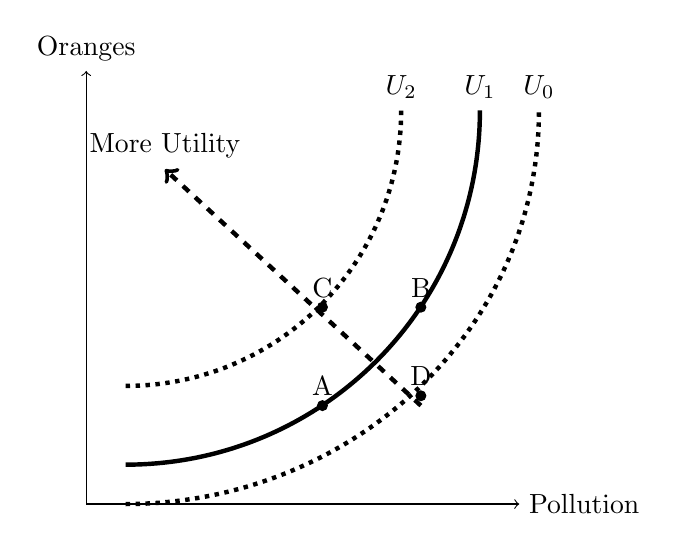
\begin{tikzpicture}[scale=.5]
			\draw[->] (0,0) -- (11,0) coordinate (x axis) node[right]{Pollution};
 			\draw[->] (0,0) -- (0,11) coordinate (y axis) node[above]{Oranges};
			\draw[ultra thick] (1,1) to[out=0, in=270] (10,10)node[above]{$U_1$};
			\draw[ultra thick, dotted] (1,3) to[out=0, in=270] (8,10)node[above]{$U_2$};
			\draw[ultra thick, dotted] (1,0) to[out=0, in=270] (11.5,10)node[above]{$U_0$};
			\draw[fill=black] (6,5) circle(0.125cm)node[above]{C};
			\draw[fill=black] (6,2.5) circle(0.125cm)node[above]{A};
			\draw[fill=black] (8.5,5) circle(0.125cm)node[above]{B};
			\draw[fill=black] (8.5,2.75) circle(0.125cm)node[above]{D};
			\draw[ultra thick, ->, dashed](8.5, 2.5)--(2,8.5)node[above]{More Utility};
 		\end{tikzpicture}
	\end{solution} 

		\part Pollution (a bad) on the horizontal axis and Garbage (a bad) on the vertical axis. 
							\begin{solution}
				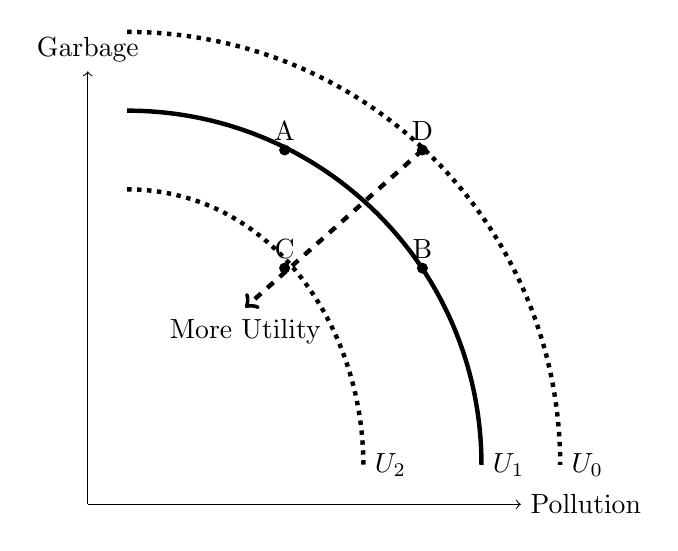
\begin{tikzpicture}[scale=.5]
			\draw[->] (0,0) -- (11,0) coordinate (x axis) node[right]{Pollution};
 			\draw[->] (0,0) -- (0,11) coordinate (y axis) node[above]{Garbage};
			\draw[ultra thick] (1,10) to[out=0, in=90] (10,1)node[right]{$U_1$};
			\draw[ultra thick, dotted] (1,8) to[out=0, in=90] (7,1)node[right]{$U_2$};
			\draw[ultra thick, dotted] (1,12) to[out=0, in=90] (12,1)node[right]{$U_0$};
			\draw[fill=black] (5,6) circle(0.125cm)node[above]{C};
			\draw[fill=black] (5,9) circle(0.125cm)node[above]{A};
			\draw[fill=black] (8.5,6) circle(0.125cm)node[above]{B};
			\draw[fill=black] (8.5,9) circle(0.125cm)node[above]{D};
			\draw[ultra thick, ->, dashed](8.5,9)--(4,5)node[below]{More Utility};
 		\end{tikzpicture}
		\end{solution} 

\part Butter on the horizontal axis and Margarine on the vertical axis. Both are goods, and you are always willing to trade between them at a 1:1 rate.

\begin{solution}
\begin{center}
	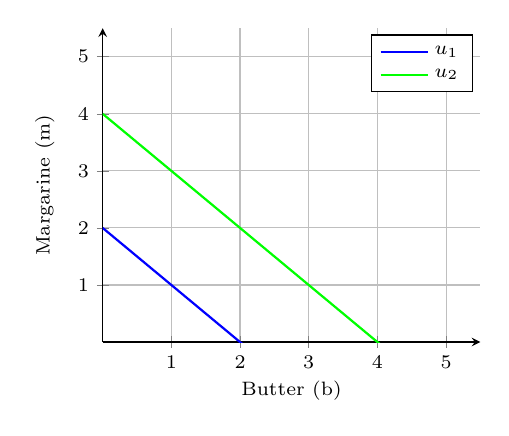
\begin{tikzpicture}\scriptsize 
	\begin{axis}[
		scale=0.7,
		axis lines=middle, 
		enlarge x limits={rel=0.1, upper},
		enlarge y limits={rel=0.1, upper},
		every axis y label/.style={at={(axis description cs:-0.2,0.5)},rotate=90,anchor=north},
		every axis x label/.style={at={(axis description cs:0.5,-0.1)},anchor=north},
	%legend pos=outer north east,
	xlabel=Butter (b),
	ylabel=Margarine (m),
	shader=flat,
	xtick={1, 2,...,5},
	ytick={0,1,...,5},
	grid=major,
	ymin=0,
	xmin=0,
	ymax=5,
	xmax=5,
]
	\addplot[domain=0:8, samples=25, thick, color=blue]{2-x};
	\addlegendentry{$u_1$}
	\addplot[domain=0:8, samples=25, thick, color=green]{4-x};
	\addlegendentry{$u_2$}
\end{axis}
\end{tikzpicture}
			\end{center}
\end{solution}

\part Cars on the horizontal axis and Tires on the vertical axis. Both are goods, and you are always want to consume them at a 1:4 proportion. (Draw these carefully!)
\begin{solution}
\begin{center}
	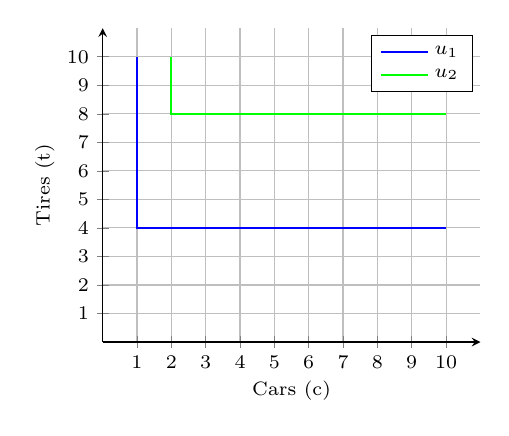
\begin{tikzpicture}\scriptsize 
	\begin{axis}[
		scale=0.7,
		axis lines=middle, 
		enlarge x limits={rel=0.1, upper},
		enlarge y limits={rel=0.1, upper},
		every axis y label/.style={at={(axis description cs:-0.2,0.5)},rotate=90,anchor=north},
		every axis x label/.style={at={(axis description cs:0.5,-0.1)},anchor=north},
	%legend pos=outer north east,
	xlabel=Cars (c),
	ylabel=Tires (t),
	shader=flat,
	xtick={1, 2,...,10},
	ytick={0,1,...,10},
	grid=major,
	ymin=0,
	xmin=0,
	ymax=10,
	xmax=10,
]
	\addplot[domain=0:8, samples=25, thick, opacity=0, forget plot]{x};
	\draw[thick, color=blue] (axis cs: 1,10)--(axis cs:1,4)--(axis cs:10,4);
	\addlegendimage{thick, color=blue};
	\addlegendentry{$u_1$}
	\draw[thick, color=green] (axis cs: 2,10)--(axis cs:2,8)--(axis cs:10,8);
	\addlegendimage{thick, color=green};
	\addlegendentry{$u_2$}
\end{axis}
\end{tikzpicture}
			\end{center}
\end{solution}
	\end{parts}

\clearpage

\question Suppose you can watch movies in the theater ($t$) and streaming at home ($s$), and earn utility according to the utility function: 
$$u(t,s)=4ts$$

Where your marginal utilities are: 
$$\begin{aligned}
MU_t&=4s\\
MU_s&=4t\\ \end{aligned}$$

\begin{parts}
\part Put $t$ on the horizontal axis and $s$ on the vertical axis. Write an equation for $MRS_{t,s}$ 
\begin{solution}
	\begin{align*}
	MRS_{t,s}&=\frac{MU_t}{MU_s}\\
	&=\frac{4s}{4t}\\
	&=\frac{4s}{4t}\\
	&=\frac{s}{t}\\
	\end{align*}
	\end{solution}
\part Would bundles of $(2,2)$ and $(1,4)$ be on the same indifference curve?
	\begin{solution}
	Simply plug in each bundle to see how much utility it generates. If they have the same utility, they are on the same indifference curve.
		\begin{align*}
		u(t,s)&=4ts\\
		u(2,2)&=4(2)(2)\\
		u(2,2)&=16\\	
		\end{align*}

		\begin{align*}
		u(t,s)&=4ts\\
		u(1,4)&=4(1)(4)\\
		u(1,4)&=16\\	
		\end{align*}
	Since both bundles generate utility of 16, they are both on the same curve.
	\end{solution}
\part Is this curve convex? Hint: Does $MRS_{t,s} \downarrow$ as $t \uparrow$? 
\begin{solution}
	We need to find the slope of the indifference curve at each bundle, and we know the slope is the MRS. If the curve is convex, the slope should decrease as we move to the right (add more $t$). 	
	\begin{align*}
	MRS_{t,s}&=\frac{s}{t}\\
	MRS_	{t,s}\bigg\rvert_{1,4}&=\frac{(4)}{(1)}\\
	MRS_	{t,s}\bigg\rvert_{1,4}&=0.25\\
	\end{align*}
	
	\begin{align*}
	MRS_{t,s}&=\frac{s}{t}\\
	MRS_	{t,s}\bigg\rvert_{2,2}&=\frac{(2)}{(2)}\\
	MRS_	{t,s}\bigg\rvert_{2,2}&=1\\
	\end{align*}
	As we get add more $t$, the MRS decreases, so the curve is convex.  
\end{solution}
\part Sketch this indifference curve. 
\begin{solution}
If we actually wanted to plot the graph correctly, take the utility function, set it equal to 16, and solve for $s$ (on the vertical axis):
\begin{align*}
u(t,s)&=4ts\\
16&=4ts\\
4&=ts\\
\frac{4}{t}&=s\\	
\end{align*}

	\begin{center} 
	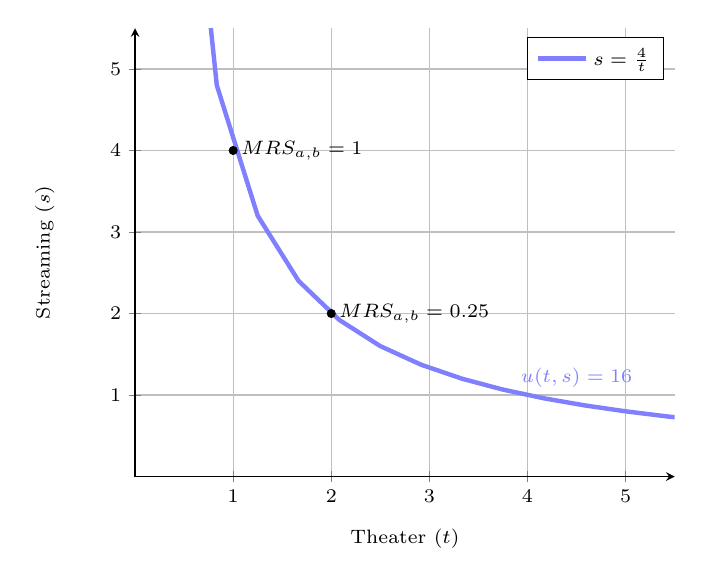
\begin{tikzpicture}\scriptsize 
	\begin{axis}[
		axis lines=middle, 
		enlarge x limits={rel=0.1, upper},
		enlarge y limits={rel=0.1, upper},
		every axis y label/.style={at={(axis description cs:-0.2,0.5)},rotate=90,anchor=north},
		every axis x label/.style={at={(axis description cs:0.5,-0.1)},anchor=north},
	%legend pos=outer north east,
	xlabel=Theater ($t$),
	ylabel=Streaming ($s$),
	xtick={1, 2,...,5},
	ytick={0,1,...,5},
	grid=major,
	ymin=0,
	xmin=0,
	ymax=5,
	xmax=5
]
	\addplot[ultra thick, color=blue!50, domain=0:10, samples=25]{4/x};
	\addlegendentry{$s=\frac{4}{t}$};
	\draw[fill=black] (axis cs:1,4)circle(0.05cm)node[right]{$MRS_{a,b}=1$};
	\draw[fill=black] (axis cs:2,2)circle(0.05cm)node[right]{$MRS_{a,b}=0.25$};
	\draw[blue!50] (axis cs:4.5,1)node[above]{$u(t,s)=16$};
\end{axis}
\end{tikzpicture}
\end{center} 
	
\end{solution}

\end{parts}

\end{questions}
\end{document}